% Created 2016-05-20 Fri 17:15
\documentclass[9pt,b5paper]{article}
\usepackage{fontspec}
\setmainfont{STSong}
\usepackage{graphicx}
\usepackage{xcolor}
\usepackage{xeCJK}
\setCJKmainfont{STSong}
\usepackage{longtable}
\usepackage{float}
\usepackage{textcomp}
\usepackage{geometry}
\geometry{left=0cm,right=0cm,top=0cm,bottom=0cm}
\usepackage{multirow}
\usepackage{multicol}
\usepackage{listings}
\usepackage{algorithm}
\usepackage{algorithmic}
\usepackage{latexsym}
\usepackage{natbib}
\usepackage[xetex,colorlinks=true,CJKbookmarks=true,linkcolor=blue,urlcolor=blue,menucolor=blue]{hyperref}


\lstset{language=c++,numbers=left,numberstyle=\tiny,basicstyle=\ttfamily\small,tabsize=4,frame=none,escapeinside=``,extendedchars=false,keywordstyle=\color{blue!70},commentstyle=\color{red!55!green!55!blue!55!},rulesepcolor=\color{red!20!green!20!blue!20!}}
\author{deepwaterooo}
\date{\today}
\title{Programming Language Theory -- Summer 2016}
\hypersetup{
  pdfkeywords={},
  pdfsubject={},
  pdfcreator={Emacs 24.5.1 (Org mode 8.2.7c)}}
\begin{document}

\maketitle
\tableofcontents


\section{Introduction}
\label{sec-1}
\begin{itemize}
\item A reposition for tracking summer2016 Programming Language Theory course.
\item Spent about two hours on <The Racket Guide> book. First 100 pages are easy, but latter on pages I just got the impression, didn't really understand all the functions, structs, objects, inheritance, package module libray etc.
\item \textbf{hw1}: A in-class demo using Racket on Wednesday evening 5/25/2016. My teammate and I are planning on some kind of animation, but have not got the final ideas yet (DrRacket Image/Rsound Animation).
\item A simple zombie house \&\& zombie are looking like:
\end{itemize}

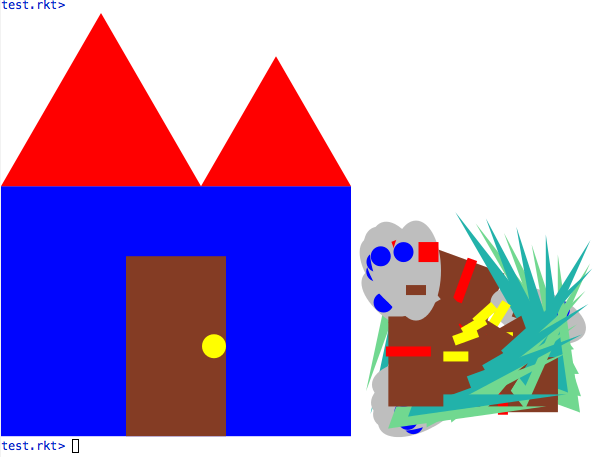
\includegraphics[width=.9\linewidth]{./pic/Screen_Shot_2016-05-20_at_5.02.01_PM.png}
\begin{itemize}
\item willl work on tetris 3d in the evening.
\end{itemize}

\section{References}
\label{sec-2}
\begin{itemize}
\item framework \url{https://github.com/NetEase/lively-logic}
\item \url{https://www.youtube.com/watch?v=SCh0zmP6R5A}
\item \url{https://www.youtube.com/watch?v=ayqhX9UA6FY}
\item \url{http://racket.tchen.me/practical-racket.html}
\item face \url{http://docs.racket-lang.org/draw/overview.html#\%28part._.Lines_and_.Simple_.Shapes\%29}
\item ͼ�Σ�\url{https://www.zhihu.com/question/20789155}
\item threads \url{http://www.ithao123.cn/content-4141200.html}
\item \url{http://docs.racket-lang.org/draw/overview.html}\#(part.\_.Lines$_{\text{and}}$\_.Simple\_.Shapes)
\item \url{http://docs.racket-lang.org/guide/classes.html}
\item \url{https://docs.racket-lang.org/quick/}
\item \url{http://docs.racket-lang.org/draw/index.html}
\item 
\item 
\end{itemize}
% Emacs 24.5.1 (Org mode 8.2.7c)
\end{document}